\documentclass[a4paper,14pt]{article} % тип документа
%\documentclass[14pt]{extreport}
\usepackage{extsizes} % Возможность сделать 14-й шрифт


\usepackage{geometry} % Простой способ задавать поля
\geometry{top=20mm}
\geometry{bottom=25mm}
\geometry{left=15mm}
\geometry{right=15mm}

\setcounter{section}{0}

%%%Библиотеки
%\usepackage[warn]{mathtext}
%\usepackage[T2A]{fontenc} % кодировка
\usepackage[utf8]{inputenc} % кодировка исходного текста
\usepackage[english,russian]{babel} % локализация и переносы
\usepackage{caption}
\usepackage{listings}
\usepackage{amsmath,amsfonts,amssymb,amsthm,mathtools}
\usepackage{wasysym}
\usepackage{graphicx}%Вставка картинок правильная
\usepackage{float}%"Плавающие" картинки
\usepackage{wrapfig}%Обтекание фигур (таблиц, картинок и прочего)
\usepackage{fancyhdr} %загрузим пакет
\usepackage{lscape}
\usepackage{xcolor}
\usepackage{dsfont}
%\usepackage{indentfirst}
\usepackage[normalem]{ulem}
\usepackage{hyperref}




%%% DRAGON STUFF
\usepackage{scalerel}
\usepackage{mathtools}

\DeclareMathOperator*{\myint}{\ThisStyle{\rotatebox{25}{$\SavedStyle\!\int\!\!\!$}}}

\DeclareMathOperator*{\myoint}{\ThisStyle{\rotatebox{25}{$\SavedStyle\!\oint\!\!\!$}}}

\usepackage{scalerel}
\usepackage{graphicx}
%%% END 

%%%Конец библиотек

\newcommand{\drawsome}[1]{            % Для быстрой вставки картинок
    \begin{figure}[h!]
            \centering
            \includegraphics[scale=0.7]{#1}
            \label{fig:first}
    \end{figure}
}
\newcommand{\drawsomemedium}[1]{
    \begin{figure}[h!]
            \centering
            \includegraphics[scale=0.45]{#1}
            \label{fig:first}
    \end{figure}
}
\newcommand{\drawsomesmall}[1]{
    \begin{figure}[h!]
            \centering
            \includegraphics[scale=0.3]{#1}
            \label{fig:first}
    \end{figure}
}

%%%Настройка ссылок
\hypersetup
{
colorlinks=true,
linkcolor=blue,
filecolor=magenta,
urlcolor=blue
}
%%%Конец настройки ссылок


%%%Настройка колонтитулы
	\pagestyle{fancy}
	\fancyhead{}
	\fancyhead[L]{Домашнее задание}
	\fancyhead[R]{Крейнин Матвей, группа Б05--005}
	\fancyfoot{}
    \fancyfoot[C]{\thepage}
    \fancyfoot[R]{ТРЯП}
%%%конец настройки колонтитулы


\begin{document}
%%%%Начало документа%%%%

\section{Задание 8}
\subsection{Задача 1}
L - язык, состоящий из всех слов в алфавите {0, 1}, которые содержат четное число нулей и нечетное число единиц.
\newline
1. Построить эквивалентную праволинейную грамматику. Будет ли она одозначной?
Построим грамматику по автомату, который принимает этот язык, мы уже строили такой в курсе,
\newline
\begin{center}
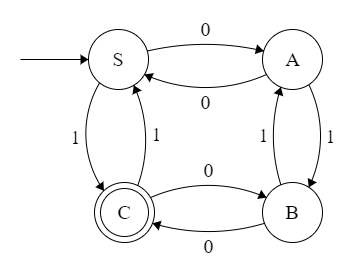
\includegraphics{03.png}
\end{center}
S $\longrightarrow$ 0A | 1C % 0 - ч, 1 - ч
\newline
A $\longrightarrow$ 0S | 1B % 0 - н, 1 - ч
\newline
B $\longrightarrow$ 0C | 1A % 0 - н, 1 - н
\newline
C $\longrightarrow$ 0B | 1S | $\varepsilon$ % 0 - ч, 1 - н
\newline
Эта грамматика будет однозначной, т.к. при каждом шаге слово, которое будет порождаться будет последовательностью каких-то терминальных символов, а на конце слова будет нетерминальный символ.
А по каждом нетерминалу переход (правило вывода) определяется однозначно, поэтому для каждого порождаемого слова будет единственный вывод.

2. При переворачивании языка L и получении $L^R$ количество единиц и нулей не изменится в нём, поэтому его будет тот же автомат, что и L.
Составим систему уравнений.
$S = 0A + 1C$ \newline
$A = 0S + 1B$ \newline
$B = 0C + 1A$ \newline
$C = 0B + 1S + \varepsilon$ \newline
Теперь осталось её решить:
\newline
$S = 0(0S + 1B) + 1(0B + 1S + \varepsilon)$
\newline
$B = 0(0B + 1S + \varepsilon) + 1(0S + 1B)$
\newline
$S = 00S + 01B + 10B + 11S + 1$
\newline
$B = 00B + 01S + 0 + 10S + 11B$
\newline
$B = (00 + 11)B + (01S + 0 + 10S)$
\newline
$B = (00 + 11)^*(01S + 0 + 10S)$
\newline
$S = 00S + (01 + 10)(00 + 11)^*(01S + 0 + 10S) + 11S + 1$
\newline
$S = (00 + (01 + 10)(00 + 11)^*(01 + 10) + 11)S + (01 + 10)(00 + 11)^*0 + 1$
\newline
$S = (00 + (01 + 10)(00 + 11)^*(01 + 10) + 11)^*((01 + 10)(00 + 11)^*0 + 1)$
\newline
РВ: $(00|(01|10)(00|11)^*(01|10)|11)^*((01|10)(00|11)^*0|1)$

\subsection{Задача 2}
Покажем индукцией по длине слова, что любое слово с равным числом букв a и b можно породить этой грамматикой.
\newline
Индукция будет по количеству терминальных символов в слове:
\newline
База: 2 S $\longrightarrow$ SS $\longrightarrow$ SSS $\longrightarrow$ SbSaS или 
$\longrightarrow$ SS $\longrightarrow$ SSS $\longrightarrow$ SaSbS. Т.е. любое слово длины 2 можно породить этой грамматикой.
\newline
Предположение: для длины 2n 
\newline
Шаг: для слова длины $2n+2$. Любое слово можно представить в виде $\omega_1 S a S b S \omega_2$ или $\omega_1 S b S a S \omega_2$.
$\omega_1 \text{и} \omega_2$ выводятся по предположению индукции, $\omega_{1_{[i]}}, \omega_{2_{[j]}} \in \{S, a, b\}$ $, i \in \overline{1,|\omega_1|}, j \in \overline{1, |\omega_2|}$.
Тогда при выводе получаем, $\omega_1 S \omega_2 \longrightarrow \omega_1 SSS \omega_2 \longrightarrow \omega_1 SaSbS \omega_2$, аналогично и для $\omega_1 SbSaS \omega_2$.
То есть мы можем вывести любое слово длины $2n+2$. Индукция доказана.

\subsection{Задача 3}
1. Покажите, что язык палиндромов в произвольном авлфавите является КС-языком.
Построим КС-грамматику, которая будет задавать язык палиндромов и докажем её корректность. Язык палиндромов = PAL.
\newline
Грамматика будет выглядеть вот так:
$\forall$ x, y $\in \Sigma^*$
S $\longrightarrow$ xSx | x | ... | ySy | y | ... | $\varepsilon$
Покажем, что $L(G) \subseteq PAL$.
\newline
Переход S $\longrightarrow$ xSx, на i-м шаге добавляет i-ое место с конца и i-ое место с начала, а переходы S $\longrightarrow$ x влияют только на середину слова.
То есть получается палиндром нечетной длины, или не добавляется символ, а добавляется $\varepsilon$ и получается палиндром четной длины. Доказано.
\newline
PAL $\subseteq L(G)$.
Любой палиндром $\omega$ нечетной длины k = 2n + 1, n $\geq 1$, можно получить, последовательно применяя правила: S $\vdash$ $ \omega_1 S \omega_1$ $\vdash \omega_1 \omega_2 S \omega_2 \omega_1$ ... $\vdash^* \omega_1 \omega_2... \omega_n S \omega_n ... \omega_2 \omega_1$ $\vdash \omega_1 \omega_2... \omega_n \omega_{n+1} \omega_n ... \omega_2 \omega_1$
\newline
Любой палиндром $\omega$ четной длины получается таким же применением правил, только в конце вместо $\omega_{n+1} ставим \varepsilon$.
S $\vdash$ $ \omega_1 S \omega_1$ $\vdash \omega_1 \omega_2 S \omega_2 \omega_1$ ... $\vdash^* \omega_1 \omega_2... \omega_n S \omega_n ... \omega_2 \omega_1$ $\vdash \omega_1 \omega_2... \omega_n \omega_n ... \omega_2 \omega_1$
Доказано.
\newline 
Получается, что L(G) = PAL. 
Получается, что язык палиндромов является КС-языком.
\newline
\underline{Доказано.}

2. Покажите, что дополнение к языку всех палиндромов тоже является КС-языком.

Построим грамматику G, дополнения к языку палиндромов. NEPAL = $\Sigma^* \ PAL$
$\forall x, y \in \Sigma^*, x \neq y$
\newline
S $\longrightarrow$ xAy | ... | yAx | ... | xSx | ... | ySy
\newline
A $\longrightarrow$ xAy | ... | yAx | ... | xSx | ... | ySy | x | ... | y | $\varepsilon$
\newline
L(G) $\subseteq$ NEPAL
Пусть ни одно слово $\omega$ из L(G) не будет палиндромом. Единственный терминальный символ, из которого можно избавиться от терминального символа будет А, а в А можно попасть только добавив различные символы справа и слева от него.
При каждом использовании этого правила мы будем дописывать по символу справа и слева от нетерминала, то есть на k-м шаге получим разные символы на k-м месте сначала и на k-м месте с конца.
А чтобы попасть в А, мы хоть раз применим правило S $\longrightarrow$ xAy | yAx , то есть будет такое k, что $\omega_i \neq \omega_{|\omega| + 1 - i}$, что по определению не будет палиндромом.
\newline
NEPAL $\subseteq$ L(G).
\newline 
Любой палиндром $\omega$ длины 2n + 1 или 2n получается последовательным применением правил:
\begin{itemize}
    \item применяем правило на k-м шаге, если $\omega_k = \omega_{|\omega| + 1 - k} = x$, S $\longrightarrow$ xSx
    \item когда на r-м шаге $\omega_r \neq \omega_{|\omega| + 1 - r}$ применим правило, $x = \omega_r, y = \omega_{|\omega| + 1 - r}$, S $\longrightarrow$ xSy
    \item потом пока $l \leq n $ если $\omega_l = \omega_{ |\omega| + 1 - l} = x$, A $\longrightarrow$ xAx, если $\omega_l \neq \omega_{|\omega| + 1 - l}$, $x = \omega_l, y = \omega_{|\omega| + 1 - l}$,, A $\longrightarrow$ xAy
    \item для последнего шага, если слово четной длины, то A $\longrightarrow \varepsilon$, если нечетной, то A $\longrightarrow \omega_{n+1}$
\end{itemize}

Получаем, что L(G) = NEPAL = $\Sigma^* \ PAL$
Получается, что язык дополнения к языку палиндромов является КС-языком.
\newline
\underline{Доказано.}

\subsection{Задача 5}
Вот детерминированный МП-автомат.
\begin{center}
    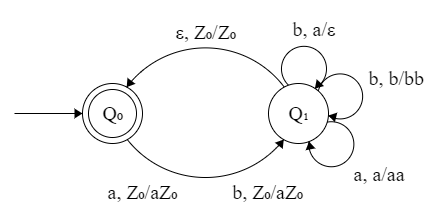
\includegraphics{04.png}
\end{center}
Докажем, что он будет принимать все слова, в которых будет одинаковое количество букв a и b.
В стеке будут находится <<лишние>> символы a, если в считанном слове было больше символов, чем b, точно также и для b. То есть в стеке сможет находится только последовательность букв aa...aaa$Z_0$, то есть разность между количеством букв a и b в считанном слове, для b аналогично.
Получим, что $Z_0$ будет находится на вершине тогда и только тогда, когда в считанном слове будет одинаковое количество букв a и b, и только тогда будет переход в принимающее состояние $Q_0$, и переход в $Q_1$, если остались еще не считанные символы.


\subsection{Задача 6}
Язык Дика с двумя типами скобок $D_2$ порождается грамматикой:

S $\longrightarrow$ SS | (S) | [S] | $\varepsilon$ 

1. Постройте недетерминированный МП-автомат, распознающий язык $D_2$.

Построим N-MA автомат $\mathcal{A}$.
\begin{center}
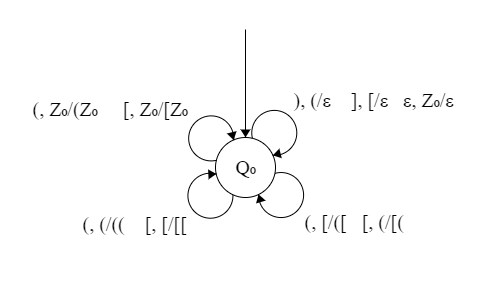
\includegraphics[scale=1]{01.png}
\end{center}

Будем доказывает, что этот автомат распознает язык Дика с двумя типами скобок.

$D_2 \subseteq L(\mathcal{A})$. Видно, что любое правильное скобочное выражение будет приниматься $\mathcal{A}$
\begin{itemize}
    \item скобочные выражения вида [], () - принимаются $\mathcal{A}$: $(Q_0, [], Z_0) \vdash (Q_0, ], [Z_0) \vdash (Q_0, \varepsilon, Z_0) \vdash (Q_0, \varepsilon, \varepsilon)$
    или же $(Q_0, (), Z_0) \vdash (Q_0, ), (Z_0) \vdash (Q_0, \varepsilon, Z_0) \vdash (Q_0, \varepsilon, \varepsilon)$.
    \item $\varepsilon$ - принимается $\mathcal{A}$: $(Q_0, \varepsilon, Z_0) \vdash (Q_0, \varepsilon, \varepsilon)$
    \item если $x \in L(\mathcal{A}), y \in L(\mathcal{A})$, то $xy \in L(\mathcal{A})$: $(Q_0, xy, Z_0) \vdash^* (Q_0, y, Z_0) \vdash^* (Q_0, \varepsilon, \varepsilon)$
    \item если $x \in L(\mathcal{A})$, то (x), [x] $\in L(\mathcal{A})$: $(Q_0, (x), Z_0) \vdash (Q_0, x), (Z_0) \vdash^* (Q_0, ), (Z_0) \vdash (Q_0, \varepsilon, Z_0) \vdash (Q_0, \varepsilon, \varepsilon)$
    или $(Q_0, [x], Z_0) \vdash (Q_0, x], [Z_0) \vdash^* (Q_0, ], [Z_0) \vdash (Q_0, \varepsilon, Z_0) \vdash (Q_0, \varepsilon, \varepsilon)$
\end{itemize}

Теперь докажем, что $L(\mathcal{A}) \subseteq D_2$. Любое слово, которое принимается $\mathcal{A}$ - правильное скобочное выражение.
\begin{itemize}
    \item $\varepsilon$ - принимается $\mathcal{A}$: $(Q_0, \varepsilon, Z_0) \vdash (Q_0, \varepsilon, \varepsilon)$ и это правильное скобочное выражение
    \item У правильных скобочных выражений итоги по [, ] и (, ) равн нулю, т.к. если открывающих скобок хотя бы одного из видов придет больше, чем закрывающих, т.е. скобочный итог по одному из видом будет положительным, то получится, что стек не будет пуст (приход открывающей скобки увиличивает число символов, которые находятся в стеке).
    \item Переходы допускают поступление закрывающей скобки какого-либо вида только в случае, если такая же открывающая скобка находится на верхушке стека, т.е. если между закрывающей и открывающей скобкой одинакого вида лежит правильное скобочное выражение.
\end{itemize}

Получаем, что $L(\mathcal{A}) = D_2$

\underline{Доказано}

2. Постройте детерминированный МП-автомат, распознающий язык $D_2$ (достаточно выполнить только этот пункт).

Построим F-MA автомат $\mathcal{A}$:

\begin{center}
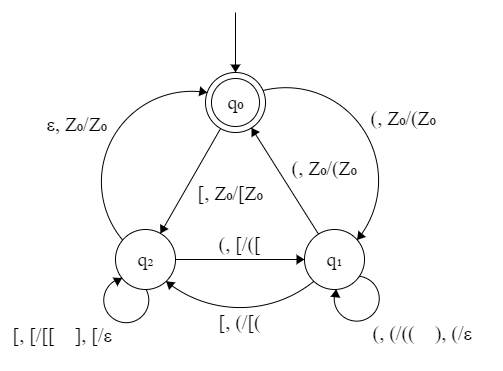
\includegraphics{02.png}
\end{center}

Докажем корректность по индукции.
$D_2 \subseteq L(\mathcal{A}_D)$
\newline
База: $\varepsilon$ - принимается. Получается, что автомат перейдет в состояние $q_0$, обработав это слово.
\newline
Шаг: пусть слово $\omega$ длины n принимается. Все правильные скобочные выражения имеют четную длину, поэтому следующий шаг будет +2.
Слово длины n+2 будет иметь один из видов: $\omega()$, $\omega[]$, $()\omega$, $[]\omega$, $(\omega)$, $[\omega]$.
Первые четыре варианта будут приниматься автомат: (), [], $\omega$ переводят автомат в принимающее состояние $q_0$.
Если слово принимается автоматом, то в стеке автомата после приема слова остается только символ $Z_0$. То есть всё, что положили в стек, досталось из него. Получаем, что в пятом и шестом случаях мы кладем в стек либо (, либо [. Потом мы кладем и выниаем из него какие-то символы из слова $\omega$, после $\omega$ остается только ( или [, потом обработаем ) или ]. Вынимаем символ из стека и можем перейти в принимающее состояние.
\newline
Шаг индукции доказан.

Получается, что любое правильное скобочное выражение принимается автоматом.
\newline
$L(\mathcal{A}_D) \subseteq D_2$
Видим, что ни одно слово, которое не будет правильным скобочным выражением, автоматом не принимается.



\end{document}